\chapter{Software Requirements Specification (SRS)}

\section{Purpose and Scope}
The purpose of Slotify is to provide a digital appointment booking system for service-based businesses that need a reliable way to manage appointments, staff schedules, and customer communication. The system is designed to support online booking, walk-in scheduling, confirmation notifications, and business-level analytics while reducing manual coordination and scheduling errors.

The scope of the project includes customer booking, staff management, business administration, automated notifications, and real-time slot validation. The application is focused on service-oriented businesses such as salons, clinics, therapy centers, and repair shops, where appointment timing and service duration are essential to daily operations.

\section{User Roles}
The system supports multiple user roles with distinct responsibilities and access rights.

\subsection{Customer}
Customers can search for businesses, view available services, select time slots, and book appointments online. They also receive confirmations and reminders and may provide feedback after a completed service.

\subsection{Business Admin}
Business administrators manage working hours, service pricing, staff profiles, and business policies. They can monitor bookings, manage staff schedules, and review business performance.

\subsection{Staff Member}
Staff members can view their assigned appointments, confirm attendance, and complete service sessions. They are also responsible for maintaining an accurate schedule for the business.

\subsection{Reception / Walk-In User}
The receptionist or front desk user can create walk-in bookings for customers who do not book online. This role helps bridge the gap between digital and physical operations.

\section{Functional Requirements}
Slotify must provide functional capabilities that support appointment booking, schedule management, communication, and reporting.

\begin{itemize}
\item The system must allow a customer to browse a business and select a service.
\item The system must display valid time slots based on business hours, staff availability, and existing bookings.
\item The system must prevent double booking through validation and database-level constraints.
\item The system must generate confirmation emails and reminder notifications.
\item The system must support the creation of walk-in appointments from the admin panel.
\item The system must allow staff and admins to manage bookings and status changes.
\item The system must support review submission after a completed appointment.
\end{itemize}

\section{Non-Functional Requirements}
The application should be reliable, fast, secure, and easy to maintain. Performance is critical during peak booking periods when multiple customers may attempt to reserve the same available time slot. Security must be enforced through authentication, role-based access control, and tenant isolation. Maintainability also matters because the system may be extended with payment integration, analytics, and mobile support in future iterations.

\begin{table}[h]
\centering
\caption{Non-functional requirements for Slotify}
\begin{tabular}{|p{3cm}|p{4cm}|p{4cm}|}
\hline
\textbf{Requirement} & \textbf{Expectation} & \textbf{Design response} \\
\hline
Performance & Slot availability must be returned quickly. & Indexed appointment queries and lightweight REST responses. \\
\hline
Reliability & A confirmed slot must not be offered twice. & Server-side validation and database-level conflict prevention. \\
\hline
Security & Users access only authorised information. & JWT authentication, role checks, and tenant-scoped data access. \\
\hline
Usability & Routine actions should be easy to complete. & Clear booking flow and role-specific dashboards. \\
\hline
Maintainability & New features should not disrupt the system. & Modular React components and controller--model--route backend structure. \\
\hline
\end{tabular}
\end{table}

\section{Use Case Diagram}
The use case model of Slotify includes actors such as the customer, business admin, staff member, and receptionist. The customer interacts with booking and review flows, while the admin and staff manage the business schedule and service execution. The receptionist supports walk-in requests and front desk operations. Together, these actors form the complete system workflow for appointment booking and service delivery.

\begin{figure}[h]
\centering
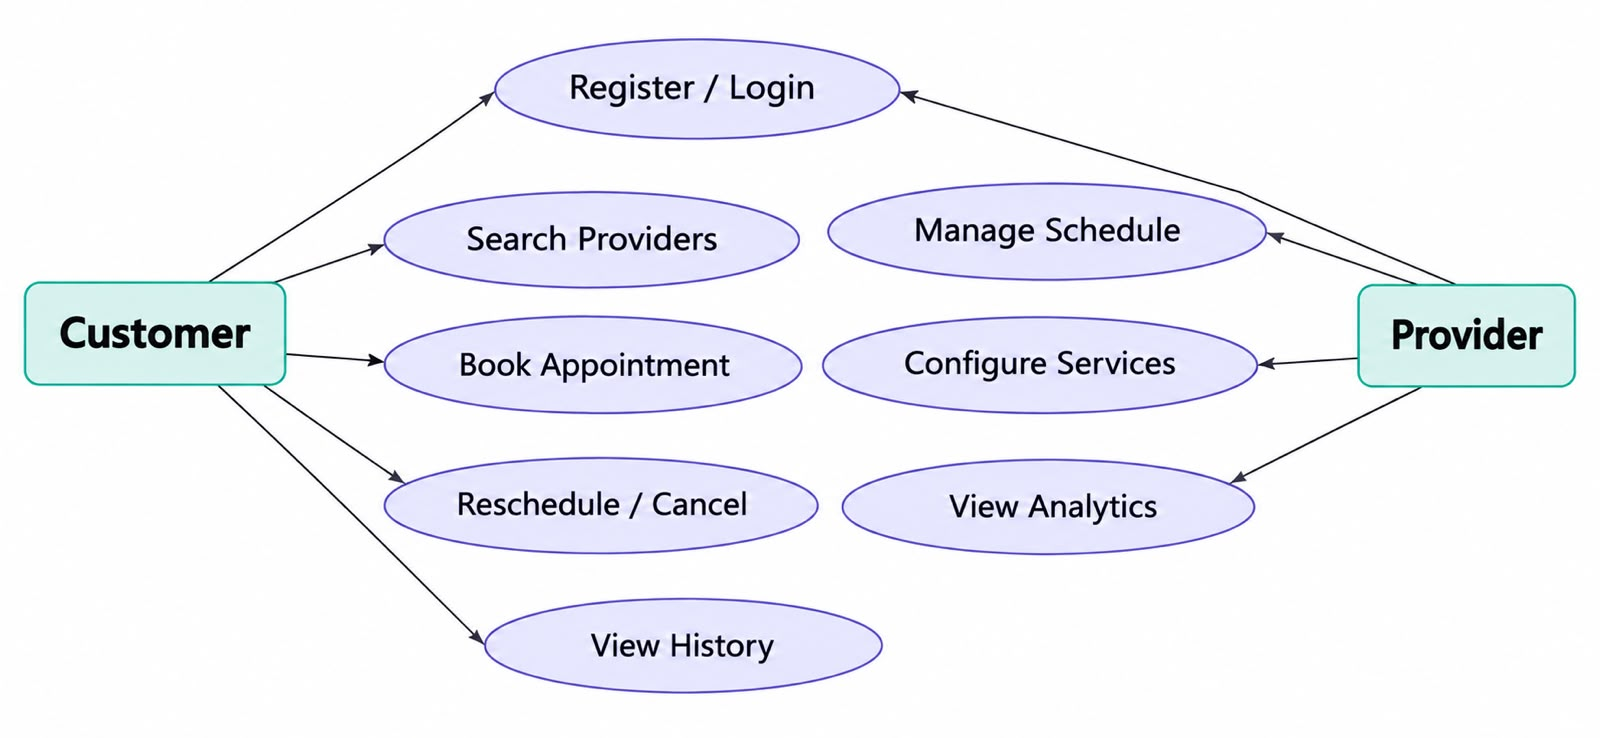
\includegraphics[width=0.9\textwidth]{images/figure 3-1.jpeg}
\caption{Use case diagram for Slotify user interactions and role-based workflow}
\end{figure}

\section{Constraints}
The system is constrained by several real-world requirements. Business schedules vary by day, staff member, and service category. The solution must therefore support flexible working hours and service-specific durations. The system also needs to operate under a multi-business environment, where data isolation and secure access are essential. In addition, the project is limited by practical implementation constraints such as time, deployment environment, and the need to keep the system simple enough for business users to adopt without technical overhead.
